\documentclass[11pt]{article}

\usepackage{fullpage}
\usepackage{graphicx}
\usepackage{amsmath}
\usepackage{amssymb}
\usepackage{amsthm}
\usepackage{fancyvrb}
\usepackage[utf8]{inputenc}
\usepackage{ragged2e}
\usepackage{subfig}
\usepackage{mathtools}
\usepackage{courier}
\usepackage{listings}
\usepackage{booktabs}
\usepackage{multirow}

\parindent0in
\pagestyle{plain}
\thispagestyle{plain}


%% UPDATE MACRO DEFINITIONS %%
\newcommand{\horrule}[1]{\rule{\linewidth}{#1}} % Create horizontal rule command with 1 argument of height

\begin{document}

\smallskip

\normalfont \normalsize 
\horrule{0.5pt} \\[0.4cm] % Thin top horizontal rule
{\centering {\huge Experiments design} \\ % The assignment title
\horrule{2pt} % Thick bottom horizontal rule

\linespread{1.5}
\justify

\section{Datasets, Algorithms and Measures}
In order to evaluate the index, we are going to use collections of real and synthetic datasets from three different sources:
\begin{enumerate}
	\item The first set of datasets is composed of 23 real datasets belonged to a publicly available outlier detection repository of approximately 1000 dataset variants from 23 main datasets\cite{campos2016}. Only one variant of each dataset was chosen. In order to select the variant of the dataset, we use the ``\textit{difficulty}'' index, that is one of the indexes proposed by the authors in this benchmark to characterize the properties of the datasets. As these datasets are originally from clustering and classification tasks and, therefore, there is no guarantee about the suitability of the labeling, this index can measure the agreement of a set of representative outlier detection methods with the labeling of the ground truth, so that a high value of index indicates that most or all methods have difficulty in finding the outliers, thus a dataset with a high value most likely does not have a consistent labeling. Consequently, only the variant with the lowest value was chosen. As the ``\textit{difficulty}'' measure cannot be used to compare dataset variants across the different outlier downsampling rates. When the dataset had variants with different outlier downsampling rates only the variants with 5\% of outliers was considered. Variants with duplicates were not considered either.
	\item The second set consists of 4 additional real world datasets: \textit{Isolet}, \textit{Multiple Features}, \textit{Optical Digits} and \textit{Vowel}. These datasets were used before in the article where IREOS was introduced\cite{marques2015}. In this article were used 11 real world datasets for the evaluation of the index, as 7 of the datasets already belong to the previously cited repository, only the other 4 were added to the experiments. 
	\item The third set is composed of 30 synthetic datasets specifically designed to evaluate outlier detection methods\cite{zimek2013}. This collection consists of two independent sets of 30 synthetic datasets each (batch1 and batch2). Only the datasets from batch1 will be used in the experiments. The datasets vary in the dimensionality $d \in [20, \dots, 40]$, in the number of clusters $c \in [2, \dots, 10]$, and for each cluster independently in the number of points $n_{ci} \in [600, \dots, 1000]$. For each cluster, the points are generated following a Gaussian model with randomly selected parameters that are attribute-wise independent. Based on the covariance matrix, the Mahalanobis distance between the mean of a cluster and each cluster point is computed. The distribution of the Mahalanobis distances follows a $\chi^2$ distribution with $d$ degrees of freedom. Those points that exhibit a distance to their cluster center larger than the theoretical 0.975 quantile were labeled as outliers, independently of the actually occurring Mahalanobis distances of the sampled points. This results in an expected amount of 2.5\% outliers per dataset. 
\end{enumerate}

In our experiments where the recommendations made by the extend IREOS is contrasted against the ground truth, we are considering Area Under the ROC Curve (ROC AUC) as the external measure to assess the quality of a given solution with respect to the ground truth.

For the purpose of the index evaluation, we collected 10 different candidate solutions for each dataset. For the real datasets, the solutions were produced by the outlier detection algorithms used in the same publicly available outlier repository where we collected the first part of the datasets\cite{campos2016}. The covered algorithms in this repository are: COF, FastABOD, INFLO, KDEOS, KNN, KNNW, LDOF, LDF, LOF, LoOP, ODIN and SimplifiedLOF. In addition to the algorithms in the repository, we also included a recent outlier detection method called GLOSH. For each dataset, each of these algorithms was performed varying its parameter value $k$ related to neighborhood size between 1 and 100. For the synthetic datasets, the solutions were produced artificially, we start from the perfect solution given by the ground truth (ROC AUC = 1) and iteratively produce new solutions replacing one of the true outliers with a random inlier. This way, at each iteration ROC AUC is reduced and we get a diverse collection of solutions to be evaluated. In order to select only the 10 different candidate solutions for each dataset (synthetic and real datasets), we collected the solutions in a way that it is the most equally distributed possibly, so we selected the best and the worst solution according to the ROC AUC and the remaining solutions were selected trying to keep an equally spaced interval among all the candidate solution for that dataset.

\section{Experiments}
We evaluate IREOS with the optional mechanism for modeling clumps $m_{cl}$ set to 1, 10, $n$. I believe use an absolute number for the intermediate value of $m_{cl}$ works better than a fraction of the size of the dataset, once small dataset will receive too small values (e.g. dataset smaller than 150 objects will receive only $m_{cl} = 1$ when used $1\%$ of dataset) and large dataset will receive too large values (e.g. dataset larger than 10.000 objects will receive $m_{cl} > 100$ when used the same $1\%$ of dataset, extreme case like KDDCup99 will receive $m_{cl} > 600$). 

\subsection{Dataset evaluation experiments}
In this experiment, we will evaluate the suitability of the real datasets from \cite{campos2016} by contrasting IREOS against the measures of difficulty and diversity. We expect the IREOS index to be negatively correlated with these measures, supporting the chose of the dataset variants by showing that datasets with small values of these measures have a more consistent labeling in agreement with IREOS. We intend to show the results in a plot such as the Figure \ref{fig:DiversityEllipses} noted with IREOS index for $m_{cl} = n$.
\begin{figure}[h!]
\center
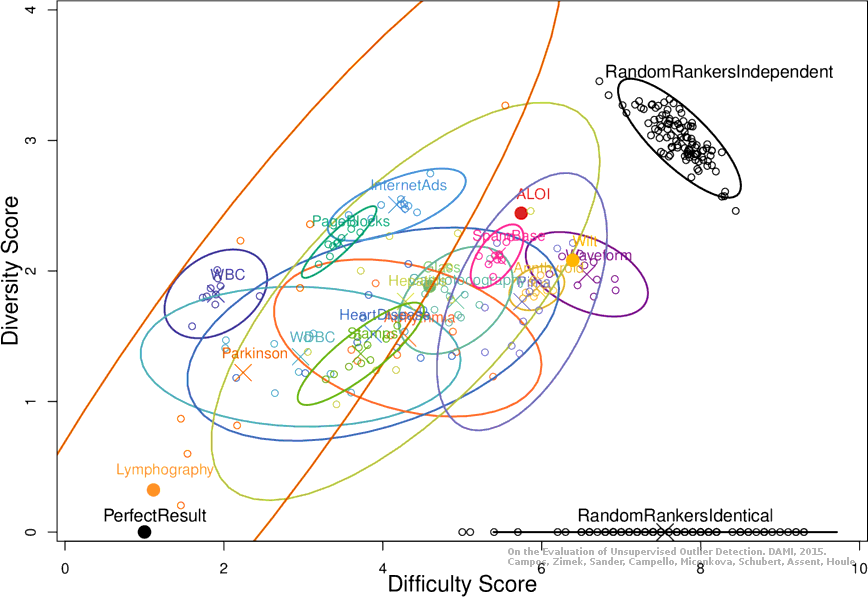
\includegraphics[width=0.5\textwidth]{figs/DiversityEllipses.png}
\captionsetup{justification=centering}
\caption{Diversity Ellipses}
\label{fig:DiversityEllipses}
\end{figure}

\subsection{Correlation experiments}\label{sec:cor}
In this experiment, we will measure the goodness of fit between the ranking obtained by assessing the solutions in a supervised way using ROC AUC and the ranking obtained by assessing the solutions in an unsupervised way using IREOS. The goodness of fit is measured by computing the Spearman correlation between these two rankings. This experiment will be run using $m_{cl} = {1, 10, n}$ for real and synthetic datasets. The results will be shown in a table such as the Table \ref{tab:cor}.
\begin{table}[]
\centering
\caption{Spearman correlation}
\label{tab:cor}
\begin{tabular}{llll}
\hline
Dataset 	& $m_{cl} = 1$ & $m_{cl} = 10$ & $m_{cl} = n$  \\ \hline
Synthetic      	& Mean $\pm$ SD & Mean $\pm$ SD  &  Mean $\pm$ SD	\\
Arrhythmia     	&   &   &  	\\ \bottomrule
\end{tabular}
\end{table}

\subsection{Model selection experiments}\label{sec:model}
In this experiment, IREOS will be applied to the set of candidate solutions, and the best solution according to the IREOS score will be selected. This solution, selected by IREOS, is then compared in terms of ROC AUC against the best ROC AUC, the worst ROC AUC, and the expected (average) ROC AUC that can be obtained in the set of candidate solutions. This experiment will be run using $m_{cl} = {1, 10, n}$ for real and synthetic datasets. The results will be shown in a table such as the Table \ref{tab:model_selection} and plot as the Figure \ref{fig:boxplot}.

\begin{table}[h!]
\footnotesize
\centering
\captionsetup{justification=centering}
\caption{Summarization of the ROC AUC values for all candidate solutions used in the experiments. Two last columns indicate the solutions selected by ext-IREOS for $m_{cl} = 1$ and $m_{cl} = n$ respectively}
\label{tab:model_selection}
\begin{tabular}{@{}llllllllll@{}}
\toprule
\multicolumn{1}{l}{Dataset} & Min & Max & \multicolumn{1}{l}{Avg} & \multicolumn{2}{l}{ext-IREOS ($m_{cl} = 1$)} & \multicolumn{2}{l}{ext-IREOS($m_{cl} = 10$)} & \multicolumn{2}{l}{ext-IREOS($m_{cl} = n$)} \\ \midrule
\multicolumn{1}{l|}{Arrhythmia}        &  0.5003   &   0.9156  & \multicolumn{1}{l|}{0.7368}    &     0.8794     & \multicolumn{1}{l|}{KNN}         &         0.8794           &       \multicolumn{1}{l|}{KNN}      & &        \\
\multicolumn{1}{l|}{WPBC}        &   0.4007  &  0.5829   & \multicolumn{1}{l|}{0.4929}    &      0.5432    & \multicolumn{1}{l|}{LDF}         &            0.5432        &       \multicolumn{1}{l|}{KNN}          & &    \\ \bottomrule
\end{tabular}
\end{table}

\begin{figure}[ht!]
\center
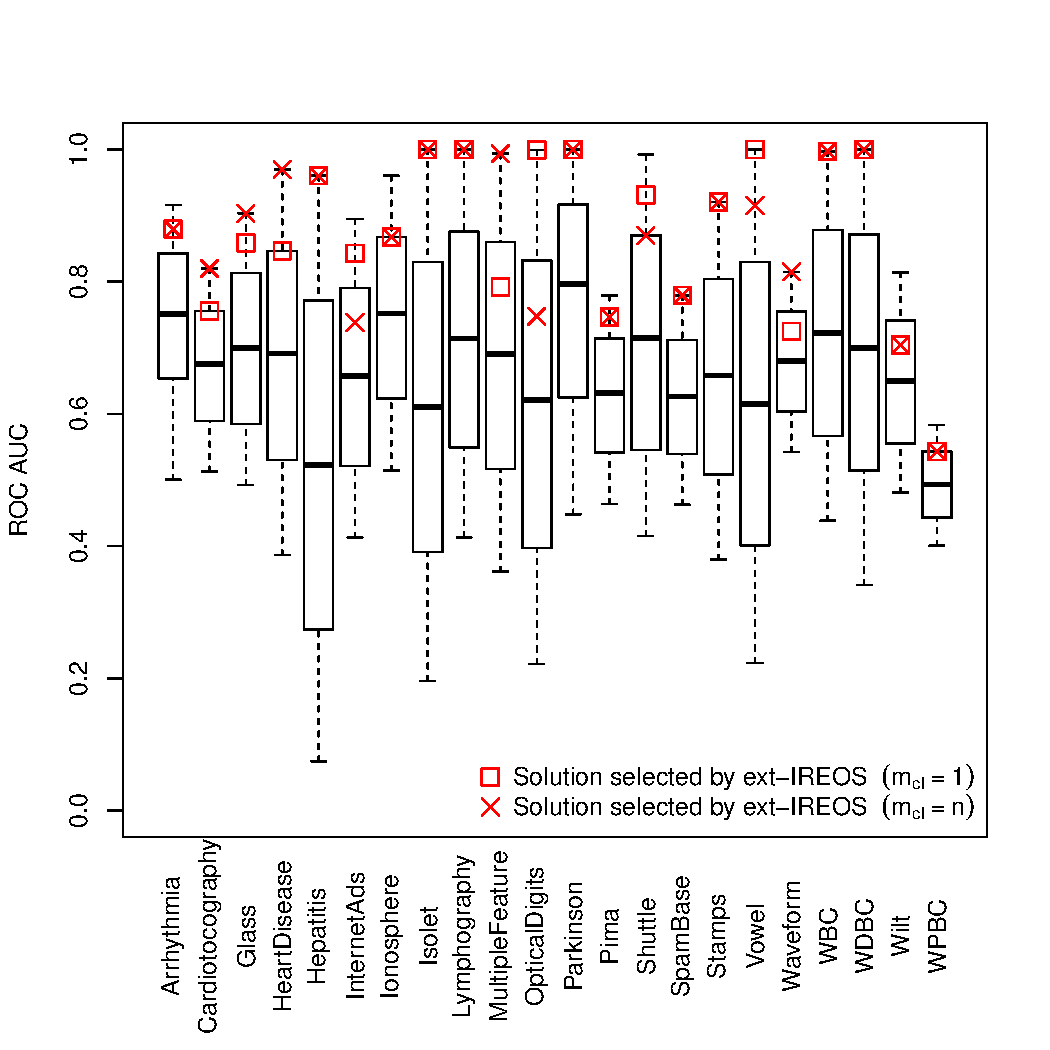
\includegraphics[width=0.5\textwidth]{figs/boxplot.pdf}
\captionsetup{justification=centering}
\caption{Distribution of the ROC AUC values for all candidate solutions used in the experiments. The position of the solutions selected by ext-IREOS for $m_{cl} = 1$ and $m_{cl} = n$ are indicated by symbols of different shapes (encoding the two values of $m_{cl}$). Some symbols are superposed.}
\label{fig:boxplot}
\end{figure}

\subsection{Computational experiments}

\subsubsection{Minimum number of $\gamma$}
In this section, we are going to perform an experiment to compare the computational cost by using a fixed number of $\gamma = 100$ to compute the separability curve, as used before in \cite{marques2015}, and use the adaptive approach. We are going to perform experiments varying the estimated error using the values: ${0.1, 0.01, 0.001}$. This experiment will be performed only in the synthetic datasets using $m_{cl} = 1$. The results will be showed in a table as the Table \ref{tab:adaptive}, where the column Total will show the total number of classifier trained to evaluate the 10 solutions of that synthetic dataset, the column Runtime will show total time spent to train the classifiers and the column Diff will show the average absolute difference from the index computed using the Original approach for the 10 solutions.

\begin{table}[h!]
\centering
\caption{Adaptive}
\label{tab:adaptive}
\begin{tabular}{|l|ll|lll|lll|lll|}
\hline
\multirow{2}{*}{Dataset} & \multicolumn{2}{c|}{Original} & \multicolumn{3}{c|}{0.1} & \multicolumn{3}{c|}{0.01} & \multicolumn{3}{c|}{0.001} \\ \cline{2-12} 
                         & Total        & Runtime        & Total  & Runtime  & Diff & Total  & Runtime  & Diff  & Total   & Runtime  & Diff  \\ \hline
                         &              &                &        &          &      &        &          &       &         &          &       \\
                         &              &                &        &          &      &        &          &       &         &          &       \\ \hline
\end{tabular}
\end{table}

\subsubsection{Separability of the minimum number of observation}
In this section, we are going to perform an experiment to compare the computational cost when compared the approach of computing the separability for all the observations and compute the separability only for the minimum possible number of observation needed. These experiments will be performed only for synthetic datasets using $m_{cl} = 1$. The results will be shown in a table as the Table \ref{tab:stopping}, where each row will be a different synthetic dataset, the column Original will show the total number of classifiers to evaluate the solutions of the given synthetic dataset when computing the separability of all data points and its runtime, the column Weights 0 will show the total number of classifiers to evaluate the solutions of the given synthetic dataset when not computing the separability for the observations with weights 0 and its runtime, and the column Stopping will show the total number of classifiers to evaluate the solutions when stopped the computation of a solution earlier because it cannot anymore surpass or by surpassed by any other solution and its runtime.

\begin{table}[h!]
\centering
\caption{Stopping}
\label{tab:stopping}
\begin{tabular}{|l|ll|ll|ll|}
\hline
\multirow{2}{*}{Dataset} & \multicolumn{2}{c|}{Original} &  \multicolumn{2}{c|}{Weights 0} & \multicolumn{2}{c|}{Stopping} \\ \cline{2-7} 
                         & Total        & Runtime        & Total  & Runtime  & Total   & Runtime    \\ \hline
                         &              &                &        &          &         &  		    \\
                         &              &                &        &          &         &        	\\ \hline
\end{tabular}
\end{table}

\subsubsection{Speed classifier up}
In this section, we are going to perform an experiment to compare the runtime when used all the observations in the dataset to compute the separability of the observations and when used only the nearest neighbor of the observation to compute its separability. We are going to perform experiments varying the number of the nearest neighbor using the absolute values: ${100, 250, 500, 1000, 2500}$. These experiments will be performed only for synthetic datasets using $m_{cl} = 1$. The results will be shown in a table as the Table \ref{tab:nn}.

\begin{table}[h!]
\footnotesize
\centering
\caption{Nearest neighbor}
\label{tab:nn}
\begin{tabular}{|l|ll|ll|ll|ll|ll|ll|}
\hline
\multirow{2}{*}{Dataset} & \multicolumn{2}{c|}{Original} & \multicolumn{2}{c|}{100} & \multicolumn{2}{c|}{250} & \multicolumn{2}{c|}{500} & \multicolumn{2}{c|}{1000} & \multicolumn{2}{c|}{2500} \\ \cline{2-13} 
                         & Index        & Runtime        & Diff     & Runtime       & Diff     & Runtime       & Diff     & Runtime       & Diff      & Runtime       & Diff      & Runtime       \\ \hline
                         &              &                &          &               &          &               &          &               &           &               &           &               \\
                         &              &                &          &               &          &               &          &               &           &               &           &               \\ \hline
\end{tabular}
\end{table}

\subsubsection{Model selection \& correlation}
The experiments \ref{sec:cor} and \ref{sec:model} will be repeated using the speed up approaches, the estimated error to compute the separability curve and the number of nearest neighbor used will depend on the results of the experiments.

\bibliographystyle{abbrv}
\bibliography{bibliography}

\end{document} 
